\documentclass{article}
\usepackage{graphicx} % Required for inserting images
\usepackage{chemfig}
\usepackage{chemformula}
\usepackage[version=4]{mhchem}
\usepackage{modiagram}
\usepackage{multirow}
\usepackage{amsmath}
\usepackage{lewis}
\graphicspath{ {./photos/} }

\title{Monopoly Problems}
\author{Andrew Ye and Diva Shah}
\date{May 2024}

\begin{document}
\maketitle
\newpage
\tableofcontents
\newpage

\section{Unit 1: Atomic Structure and Properties}
\subsection*{Problem 1}
Calculate the number of moles in a \(7.89 kg\) sample of \(\ce{C_9H_8O_4}\) 
\subsection*{Problem 2}
Given this graph, what is true about the element depicted
\begin{center}
    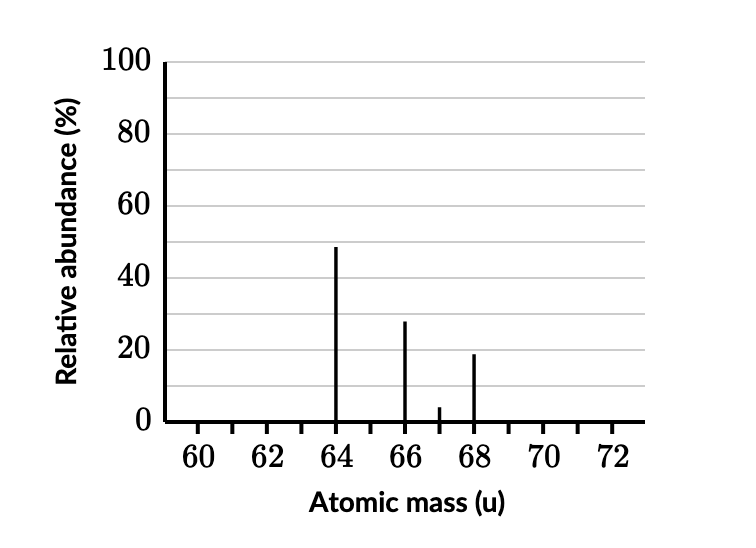
\includegraphics[scale = 0.5]{photos/photo1.png}
\end{center}
(a) In an average sample of the element, less than \(20\%\) of the atoms have an atomic mass of \(66u\). \\
(b) The most abundant isotope of the element has an atomic mass of \(64u\). \\
(c) The element has an average atomic mass of \(64u\). \\
(d) The element has an average atomic mass between \(66\) and \(68u\). \\
\subsection*{Problem 3}
What is the percent composition of Carbon in \(\ce{C_{13}H_{18}O_2}\)?


\newpage
\section{Answers}
\subsection{Unit 1}
\subsubsection*{Problem 1}
The molar mass of \(\ce{C_9H_8O_4}\) is \(1.008*8 + 12.01*9 + 16.00*4 = 180.2 \frac{g}{mol}\)
\begin{equation}
\begin{aligned}
    7.89kg \times \frac{1g}{10^{-3}kg} \times \frac{1mol}{180.2g} = 43.8mol
\end{aligned}
\end{equation}
\subsubsection*{Problem 2}
(b), the tallest peak of the graph is the one at \(64u\). 
\subsubsection*{Problem 3}
In one mole of \(\ce{C_{13}H_{18}O_2}\) is \(206.31g\).
\begin{equation}
\begin{aligned}
    1mol\hspace{0.1em}\ce{C_{13}H_{18}O_2} \times \frac{13mol\hspace{0.1em}\ce{C}}{1mol\ce{C_{13}H_{18}O_2}} \times \frac{12.01g}{1mol\hspace{0.1em}\ce{C}} = 156.31g
\end{aligned}
\end{equation}
Thus, the percent composition by weight is \(\frac{156.31}{206.31} = 75.764\%\)



\end{document}